% vim: tw=80 noai
\documentclass[normaltoc,capchap,capsec,times]{abnt}
%\usepackage{t1enc}
%\usepackage[latin1]{inputenc}
%\usepackage[T1]{fontenc}
\usepackage[utf8]{inputenc}
\usepackage[brazil]{babel}
\usepackage[alf]{abntcite}
\usepackage[ordem=alf]{tabela-simbolos}
\usepackage{url}
\usepackage{graphicx}
\usepackage{listings}
\usepackage{verbatim}
\usepackage{subfigure}
\usepackage{multicol}
\usepackage{framed}
\def\lstlistingname{Listagem}

%%%%%%%%%%%%%%%%%%%%%%%%%%%%%%%%%%%%%%%%%%%%%%%%%%%%
% Dados da monografia
%%%%%%%%%%%%%%%%%%%%%%%%%%%%%%%%%%%%%%%%%%%%%%%%%%%%

\newcommand{\meunome}{Ivan Carmo da Rocha Neto}
\newcommand{\meutitulo}{Navi: Sistema para Gerenciamento de Informações e Execuções de Análise Filogenética Através de Redes Complexas}
%\newcommand{\meusubtitulo}{Uma abordagem focada na experiência do usuário}
\newcommand{\meuano}{2011.2}
\newcommand{\meuorientador}{Orientador: \prof\ Antonio Lopes Apolinário Jr.}

%%%%%%%%%%%%%%%%%%%%%%%%%%%%%%%%%%%%%%%%%%%%%%%%%%%%

%% O comando \obs aqui definido permite que o autor faca anotacoes na
%% monografia que aparecem no PDF gerado. Para ativar o comando, descomente
%% a primeira linha e comente a segunda.
%% Exemplo de uso: \obs{Preciso melhorar este pargrafo...}

%\newcommand{\obs}[1]{\underline{\textbf{OBSERVAO}}: \emph{#1}}
\newcommand{\obs}[1]{}

\def\ordfem{\mbox{\raise .35em \hbox{\underline{\scriptsize a}\ }}}
\def\ordmasc{\mbox{\raise .35em \hbox{\underline{\scriptsize o}\ }}}
\def\profa{Prof\ordfem.}
\def\prof{Prof\ordmasc.}

%%%%%%%%%%%%%%%%%%%%%%%%%%%%%%%%%%%%%%%%%%%%%%%%%%%%

\begin{document}

% Capa com Braso

\begin{titlepage}
   \begin{center}
    	%logotipo
               
\includegraphics{brasaoUFBA} \\
	%\vspace{0.7in}
              \centering{ 
	      \bf{
	      \LARGE{
		\uppercase{UNIVERSIDADE FEDERAL DA BAHIA} \\
 	      }
	      \Large {
                   	\uppercase{INSTITUTO DE MATEMÁTICA} \\
	      }
                   \large {
                       \uppercase{DEPARTAMENTO DE CIÊNCIA DA COMPUTAÇÃO} \\
                  }
              } }
   \end{center}
   \vfill
   \begin{center}
       \bf{
       \large{\uppercase{\meunome}  \\  }
       }
   \end{center}
   \vspace{0.2in}
   \begin{center}
       \bf{
      	 \LARGE{ \uppercase{\meutitulo} } \\
      	 %\Large{ \uppercase{\meusubtitulo} }
         \obs{\\ \Large{Esta verso da monografia contm comentrios do autor.
          Para remov-los, redefina o comando LaTeX \texttt{obs}.}}
       }
   \end{center}

   \vfill
   \hspace{\stretch{1}}
   \vfill
   \begin{center}
      \normalsize{
          Salvador \\
          \meuano
       }
   \end{center}

\end{titlepage}

%comando abaixo cria uma capa redundante, mas como a capa com braso foi 
% feita 'manualmente', no faz sentido usar este comando:
%\capa



%\folhaderosto
% o comando acima foi comentado para no criar uma folha de 
% rosto redundante, j que ela feita 'manualmente' abaixo

\begin{titlepage}
 \vfill
 \begin{center}
   {\large \uppercase{ \bf{ \meunome\ } } } \\[7cm]
   {\Huge \uppercase{ \bf{ \meutitulo\ } } }\\[1cm]
   \vfill
   \hspace{.45\textwidth} % posicionando a minipage
   \begin{minipage}{.5\textwidth}
     \begin{espacosimples}
       \bf{
	Monografia apresentada ao Curso de gradução em Ciência da Computação, 
	Departamento de Ciência da Computação, Instituto de Matemática, Universidade Federal da 
	Bahia, como requisito parcial para obtenção do grau de Bacharel em Ciência da Computação. \\ 
       }      
     \end{espacosimples}
     \begin{espacosimples}    
       \meuorientador
       \newline
       \meucoorientador
     \end{espacosimples}
   \end{minipage}
   \vfill
   Salvador \\
   \meuano
 \end{center}
\end{titlepage}


\begin{resumo}
O método de análise filogenética através de redes complexas parte de princípios teóricos da Física Estatística e utiliza técnicas computacionais
baseadas em Teoria dos Grafos, se mostrando como uma alternativa viável aos pesquisadores, à medida em que se equipara a outros métodos quanto à qualidade
dos resultados. Neste trabalho de análise e desenvolvimento são organizados os dados, informações e programas desenvolvidos pelo grupo FESC (Física
Estatística e Sistemas Complexos - Instituto de Física - UFBA), e é projetado um \textit{software} visando a facilidade de uso por biólogos, físicos
e bioinformáticos como uma importante alternativa às ferramentas existentes para análise filogenética, se utilizando das melhores práticas de
Engenharia de Software, incluindo análise de requisitos, modelagem de classes e de interações entre os usuários e o sistema, beneficiando pesquisadores
pela própria organização do processo e isenção dos usuários de algumas preocupações referentes ao mesmo, além de também tornar possível a continuação
de seu desenvolvimento e manutenção de forma facilitada.

\textbf{Palavras-chave:}
análise filogenética,
engenharia de software, 
reengenharia,
modelagem,
desenvolvimento.
\end{resumo}

% O abstract e' opcional.
\begin{abstract}
The method of phylogenetic analysis through complex networks comes from the theoretical principles of Statistical Physics and uses computational
techniques based on Graph Theoryis, shown as an feasible alternative for researchers, to the extent that it matches the other methods on the quality of
results. In this work of analysis and development data, information and programs development by FESC (Group of Statistical Physics and Complex Systems - 
Physics Institute - UFBA), and a software are organized in order to get ease of use bt biologists, physicists and bioinformatics as an important
alternative to existing tools for phylogenetic analysis, with the use of best practices of Software Engineering, including requirements analysis,
modeling classes and interactions between users and the system, benefiting researchers by the organization of the process and exemption
for users of some concerns referring to it, and also make possible the continuation of its development and maintenance of an easier way.

\textbf{Keywords:} 
phylogenetic analysis,
software engineering,
reengineering,
modeling,
development
\end{abstract}

%% As listas a seguir sao opcionais:
\listadefiguras
%\listadetabelas
\listadesiglas
%\listadesimbolos

\sumario

% O conteudo da monografia esta' nos seguintes arquivos:
\chapter{Introduo}

Modelo de monografia usando as normas ABNT (Associao Brasileira de Normas
Tenicas) \sigla{ABNT}{Associao Brasileira de Normas Tenicas}
e adaptao personalizada 
do padro do Departamento de Cincia da Computao (DCC) da Universidade
Federal da Bahia (UFBA).
\sigla{DCC}{Departamento de Cincia da Computao}
\sigla{UFBA}{Universidade Federal da Bahia}
Fontes latex cedidos pela ABNT e disponibilizados por 
Maurcio Vieira. (Valeu Maurix!). Adaptado por Abelmon Bastos por solicitao
da \profa\ Dbora Abdalla para o semestre 2005.1.
Adaptado por Rodrigo Rocha por solicitao da \profa\ Dbora Abdalla no fim
do semestre 2007.1.

% use sua propria estrutura

%Problema etc

%Objetivo etc

%Resultados esperados etc

%Estrutura/Organizao etc

\chapter{Análise Filogenética através de Redes Complexas} \label{cap:analisefilo}

Análise Filogenética é uma área da Biologia que tem despertado bastante interesse pelos pesquisadores. A evolução do poder de processamento dos computadores
permitiu que se pudesse comparar sequências proteicas ou nucleotídicas muito rapidamente, gerando um poder de análise abrangente no que tange as relações entre
proteinas, enzimas, rotas metabólicas e consequentemente seres vivos. Essas análises, por conseguinte, geraram descobertas importantes que influenciaram o
modo como enxergamos a evolução das espécies e a relação entre elas em geral.

Atualmente existem quatro métodos bem aceitos na literatura para Análise Filogenética: Análise Bayesiana \textbf{[CITAR]}, Análise de Parcimônia
\textbf{[CITAR]}, Análise de Distâncias \textbf{[CITAR]} e Análise por Verossimilhança \textbf{[CITAR]}. Estas análises partem de alguns pressopostos
biológicos, que são informações iniciais necessárias a sua realização. O uso da Física Estatística para tratar os dados referentes a proteinas de
determinadas rotas metabólicas permite o desenvolvimento de um método que não necessite desses pressupostos.

A área de Física Estatística atualmente apresenta forte caráter interdisciplinar, permitindo a modelagem e análise de diversos sistemas
que englobam outras áreas de conhecimento. A aplicação da Teoria das Redes Complexas em Bioinformática, apoiada pela Teoria dos Grafos,
juntamente com conhecimentos de Física, Matemática e Biologia vem se mostrando como uma alternativa interessante na modelagem de sistemas biológicos,
e serviu para que o FESC (Física Estatística e Sistemas Complexos - Instituto de Física - UFBA) desenvolvesse um método para Análise Filogenética.

Como foi dito anteriormente, o objetivo deste trabalho é controlar o processo e fornecer um ambiente para o armazenamento de informações em relação às
execuções, além de uma interface de fácil utilização para um pesquisador da área de Biologia. A figura \ref{fig:fluxograma} mostra o fluxograma geral
sobre os passos da execução do método. As seções que seguem explicam estes passos com mais detalhes.

\begin{figure}
\centering

\includegraphics{brasaoUFBA2}
\caption{Fluxograma com os passos da execução do método de análise filogenética desenvolvido pelo FESC.}
\label{fig:fluxograma}
\end{figure}


\section{Escolha de Sequências Proteicas} \label{sec:escseq}

A primeira etapa do método consiste na escolha das sequências que serão utilizadas para a construção e caracterização da rede.
Usualmente a escolha é feita a partir de um banco de dados biológico, disponível livremente pela web. Durante todo o trabalho na utilização
do método, as sequências escolhidas vieram do NCBI \cite{ncbi}, um banco de dados bastante utilizado no meio biológico, que contém dados de sequências
nucleotídicas e sequências proteicas, entre várias outras informações. A escolha das sequências proteicas é feita utilizando como critério
uma rota metabólica, separando as sequências pela enzima que as produzem na rota.

\sigla{NCBI}{National Center for Biotechnology Information}

Esta é uma etapa manual, onde são feitas buscas por data e são realizadas determinadas filtragens no site do NCBI para obter as sequências desejadas. O
sistema desenvolvido neste trabalho leva em consideração que as sequências já foram escolhidas e as recebe como entrada inicial. O resultado desta etapa
são arquivos no formato GenBank (NCBI) que são filtrados e organizados para facilitar a identificação de organismos em etapas posteriores e proporcionar
a execução da similaridade. Um requisito importante então é a capacidade de receber um ou mais arquivos naquele formato e a partir deles realizar uma
filtragem e gerar a matriz de similaridades.

\section{Similaridade} \label{sec:similaridade}

Para executar a análise de similaridades entre as sequências proteicas, a partir da filtragem realizada no passo anterior e o armazenamento em um banco
de dados relacional, é utilizada ferramenta BLAST (Basic Alignment Search Tool) \cite{blast1997} para comparação entre as sequências. O BLAST trabalha
tanto com sequências nucleotídicas quanto proteicas. O interesse do uso do BLAST para o método em questão está na comparação de sequências proteicas
utilizando o alinhamento local, que compara duas sequências isoladamente e retorna uma porcentagem de similaridade entre elas.

\sigla{BLAST}{Basic Alignment Search Tool}

A partir do resultado do BLAST, pode-se construir uma matriz de similaridades \cite{andrade2006}, onde as linhas e colunas representam as sequências e
uma posição $(i, j)$ da matriz armazena a similaridade entre elas. Desta matriz são construídas as redes que caracterizam as sequências, que serão
descritas na próxima seção.

\section{Construção e Caracterização das Redes} \label{sec:conscarac}

O conceito de rede está associado ao de um grafo, que é um par $G = (V, E)$ de conjuntos onde $E \subseteq [V]^2$, então os elementos de $E$
são subconjuntos de dois elementos de $V$. Para evitar ambiguidades de notação, devemos assumir que $V \cap E = \O{}$. Os elementos de $V$ são os vértices
(ou nós ou pontos) e os elementos de $E$ são suas arestas (ou linhas) \cite{reinhard2010}.

Podemos dizer que o estudo de uma rede é o estudo de um grafo, mas em uma escala maior. Redes podem ser tidas como grafos muito grandes e complexos,
em que se torne mais preciso o uso de técnicas estatísticas para a sua análise \cite{bessa2008}. Na literatura de Redes Complexas, em geral, precisamos
encontrar uma rede de determinado conjunto que melhor caracterize este conjunto. Essa escolha se dá pela relação entre ruído e informação \cite{barabasi2004}.

Partindo da matriz de similaridades, podemos construir até 101 (similaridade 0\%-100\%) matrizes de adjacência, se levarmos em consideração que podemos
escolher um valor limiar e construir a rede baseada nele. Por exemplo, se escolhermos o valor 60 como limiar, construiremos uma rede onde haverá uma aresta
entre dois vértices (sequências) se e somente se a similaridade entre eles em questão for maior ou igual a 60. Uma rede com limiar muito baixo apresenta muito
ruído (muitas arestas, pouca possibilidade de identificação de suas características) e uma rede com limiar muito alto apresenta pouca informação (poucas
arestas, também pouca possibilidade de identificação de suas características).

Como resultado, temos 101 redes (grafos) representados pelas matrizes de adjacência, que foram geradas a partir da conexão de pares de vértices que
têm uma similaridade maior ou igual a um valor limiar.

Partindo das matrizes de adjacência podemos também criar matrizes de vizinhança \cite{andrade2009}, que podem ser obtidas calculando-se os caminhos mínimos
\cite{bessa2008} entre os vértices da rede ou através da multiplicação booleana de matrizes de adjacência de ordens consecutivas \cite{andrade2006}. Na figura 
\ref{fig:matriz-vizinhanca}, temos um exemplo de matriz de vizinhança, onde cada cor representa um valor de distância entre dois vértices. Pela figura, temos
que se a distância entre dois vértices é 1, o ponto que representa a relação entre eles recebe a cor azul escura. Se for 7, por exemplo, receberá a cor
amarela.

Alguns \textit{softwares} utilizados geram as matrizes em memória e as excluem após determinados cálculos, e outros simplesmente as salvam em certa estrutura
de diretórios. A possibilidade de dar ao usuário o poder de gerenciar essas matrizes e realizar operações diversas, como compará-las ou visualizar gráficos
a partir delas dentro de um projeto é algo importante que deve estar incluído no modelo.

\begin{figure}
\centering
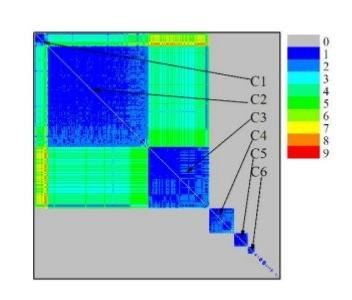
\includegraphics[scale=0.53]{matriz-vizinhanca}
\caption{Exemplo de Matriz de Vizinhança no formato de Matriz de Cores.}
\label{fig:matriz-vizinhanca}
\end{figure}

\section{Limiar Crítico} \label{sec:limcrit}

Já se sabe que o limiar crítico de uma rede revela a melhor relação entre ruído e informação. Existem diversas maneiras de se determinar o limiar
crítico da rede. Uma delas, utilizada pelo FESC, é o método das distâncias \cite{andrade2011}. Nele, calcula-se a distância euclidiana entre matrizes de
vizinhança de limiares consecutivos \cite{andrade2008}. A matriz que apresentar a maior distância entre a de limiar conscutivo
ao seu será a escolhida como a matriz do limiar crítico, para representar a rede. É necessário escolher a melhor rede que representa o conjunto.
A rede do limiar crítico cumpre bem este papel.

Na figura \ref{fig:distancia}, temos o exemplo de um resultado do cálculo das distâncias entre matrizes de vizinhança, onde o limiar crítico é representado
pelo pico do gráfico, ou seja, o valor 51. A rede que representa todo o conjunto é então a rede do limiar 51, que será utilizada na última etapa do processo,
que é a clusterização, que utiliza um conceito chamado entremeação.

O método das distâncias pode ser utilizado para a determinação do limiar crítico, mas isto pode ser feito através de outros métodos, como a verificação da
variação do tamanho do maior \textit{cluster} da rede em função da variação do limiar. O processo poderia fornecer a possibilidade de escolha do método de
análise dos limiares. Além disso, é importante a geração dos gráficos dos resultados destas execuções e exibição para o usuário, eliminando a possibilidade
de trocas de contexto (como reinicialização da máquina, mudança de sistema operacional ou de \textit{software}) que atrasam o prosseguimento do processo.

\begin{figure}
\centering
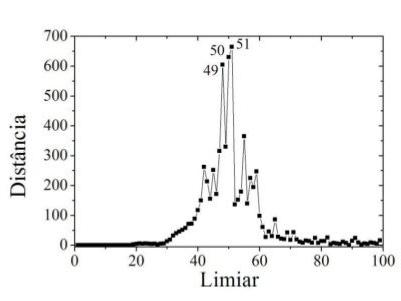
\includegraphics[scale=0.58]{distancia}
\caption{Resultado da execução do método das distâncias entre limiares consecutivos, resultando em um gráfico Distância x Limiar.}
\label{fig:distancia}
\end{figure}

\section{Entremeação e Centralidade} \label{sec:entremeacao}

A Matriz de Vizinhança da rede do limiar crítico é a entrada necessária para a realização da clusterização, que é feita através do método de detecção
de comunidades de Newman e Girvan \cite{newman2004} para identificar a estrutura modular da rede. O método consiste em determinar a aresta mais importante
da rede – aquela por onde passa a maior quantidade de caminhos mínimos de cada par de vértices por toda a rede – e eliminá-la, repetindo a operação
até que não existam mais arestas na rede.

Conforme a operação é feita, é possível construir um histograma de remoção de arestas ou dendrograma, que começa com uma linha representando toda a rede
e à medida em que a rede vai aumentando o número de partes desconexas da mesma com a remoção de arestas, a linha relativa à parte da rede que se quebrou
se subdivide em duas. O dendrograma auxilia na identificação de comunidades e propicia as análises biológicas dos resultados, além da comparação com outros
métodos da Biologia, visto que seu formato de árvore em que as linhas mais à direita representam cada uma das sequências proteicas (vértices da rede)
é também o formado de saída dos outros métodos de Análise Filogenética. A figura \ref{fig:dendrograma} mostra com detalhes um exemplo de dendrograma
para o limiar crítico 51.\newline

Para a geração do dendrograma é necessária a escolha do limiar pelo usuário, e seu algoritmo recebe como entrada a matriz de vizinhança referente a este
limiar, que em um sistema deve estar armazenada. A execução desta etapa é a mais demorada, variando de cinco minutos a mais de três meses, a depender do
tamanho da rede. 

\begin{figure}
\centering
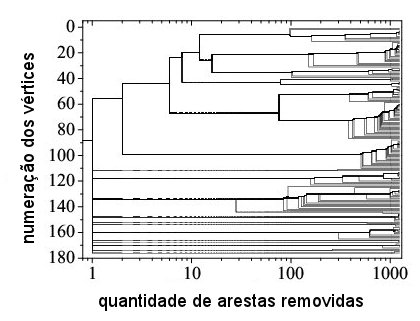
\includegraphics[scale=0.73]{dendrograma}
\caption{Exemplo de dendrograma para o limiar crítico 51.}
\label{fig:dendrograma}
\end{figure}

O método completo em questão é explicado com mais detalhes em \cite{goesneto2010} e \cite{andrade2011}. Ele utiliza uma determinada quantidade de programas,
cada um seguindo certos padrões de entrada e saída, além de arquivos de configuração.
Tais características dificultam sua utilização por pesquisadores de outras áreas que não Física ou Ciência da Computação, além de trazê-los uma preocupação
desnecessária com localização e distribuição de arquivos. Para um melhor aproveitamento do método, seria mais interessante que o controle do processo de
execução fosse realizado por um sistema, dispondo de um ambiente de fácil utilização e que realizasse o gerenciamento das informações por meio de uma camada
de persistência, deixando a questão da organização dos dados transparente para o pesquisador.

O processo pode então ser resumido tecnicamente como uma série de execuções de programas que recebem arquivos de entrada em determinado formato, realizam um
processamento e geram um arquivo de saída. Os requisitos mais importantes, portanto, são a eliminação da necessidade de organização de arquivos intermediários
pelos usuários e a conversão de formatos entre as execuções. Para agilizar aa execução, é importante também a geração de gráficos em determinadas etapas. A
tabela \ref{tab:requisitos} mostra os requisitos necessários para a construção do Navi - Sistema para Gerenciamento de Informações e Execuções de Análise
Filogenética Através de Redes Complexas.

\begin{table}
\centering
\caption{Tabela de requisitos do Navi} % igual ao ambiente figura
\begin{tabular}{p{5cm}p{10cm}} % com este comando dizemos quantas colunas terá nossa tabela e a posição do texto dentro de cada coluna. Aqui temos três colunas (pois são três "c" dentre {}) e o texto estará centralizado em todas elas (indicado pelo "c", se quisermos alinhados à esquerda "l" ou direita "r"
\hline 
%Requisito & Pontos & Classificação \\
Requisito & Descrição \\ 
\hline
\hline
%Cruzeiro & 52 & 1 \\
%Sao Paulo & 50 & 2 \\
%Gremio Barueri & 47 & 3 \\
Filtragem de arquivos no formato GenBank & O sistema deve receber um diretório e ler dele arquivos no formato do GenBank, e a partir deles criar os organismos,
as sequências com nome, identificador, código e outras informações\\ \hline
Controle do projeto & O sistema deve prover ao usuário a possibilidade de criar, salvar ou carregar um projeto. \\ \hline
Salvar os organismos e sequências & O sistema deve salvar os organismos e as sequências para posterior consulta. Deve ser criada uma estrutura de
armazenamento que livre o usuário da necessidade de instalar sistemas de bancos de dados relacionais \\ \hline
Escolha de sequências & O sistema deve permitir a escolha de sequências para a geração da matriz de similaridades \\ \hline
Gerar matrizes de adjacência & O sistema deve gerar matrizes de adjacência com base no limiar fornecido pelo usuário, também mostrando o gráfico de uma
forma opcional \\ \hline
Gerar matrizes de vizinhança & O sistema deve gerar matrizes de vizinhança com base no limiar fornecido pelo usuário, também mostrando o gráfico de uma
forma opcional \\ \hline
Analisar limiares & O sistema deve fornecer opções de métodos para a análise de limiares, mostrando obrigatoriamente o gráfico como resultado\\ \hline
Executar clusterização & O sistema deve fornecer opções de métodos de clusterização, que depende da escolha de um limiar pelo usuário, além de mostrar o
gráfico de seu resultado quando requisitado \\ \hline
Visualizar gráfico completo da rede & O sistema deve permitir a visualização do gráfico completo da rede, após a escolha das comunidades, recuperando as
informações salvas durante o processo de salvamento das sequências e organismos \\ \hline
Congruência & O sistema deve permitir a comparação do resultado do método com o resultado de outros métodos de análise filogenética, além da comparação
com o resultado pelo próprio método com outro conjunto de dados \\ \hline
Exportar dados & O sistema deve permitir a exportação de dados necessários à geração de gráficos para o uso pelos usuários de ferramentas profissionais de
plotagem \\ \hline
\end{tabular}
\label{tab:requisitos}
\end{table} 

A partir desses requisitos gerais, o sistema Navi será modelado, o que é mostrado no próximo capítulo.


\chapter{Modelagem do Navi - Sistema para Gerenciamento de Informações e Execuções de Análise Filogenética Através de Redes Complexas}
\label{cap:navi}

O processo descriito no capitulo anterior envolve diversos modulos independentes com diferentes padrões de entrada e saída, e formas de configuração. Tal
fato dificulta bastante sua execução e o controle dos diversos conjuntos de dados gerados em cada etapa do processo, bem como dos parametros que os originaram.
Portanto, o desenvolvimento de um sistema para gerenciar o método de Análise Filogenética por Redes Complexas descrito anteriormente precisa seguir três
importantes pilares:

\begin{itemize}
 \item{Usabilidade é um fator importante por tornar o método passível de utilização por pessoas com pouco ou quase nenhum conhecimento de programação neste
caso específico, e para gerar uma boa experiência do usuário e fazer com que seu uso seja agradável no caso geral. Segundo \cite{nielsen1993}, interfaces de
usuário são uma parte muito mais importante para computadores em geral do que já foram um dia, e hoje respondem por mais de 45\% do código-fonte de um
\textit{software}.}
  \item{Organização torna possível a criação, importação e exportação de projetos contendo as execuções necessárias para as análises,
onde os dados podem ser agrupados em um formato de arquivo possível de ser transportado entre múltiplas máquinas e contendo todas as informações
necessárias para a retomada de execuções.}
  \item{Transparência, não menos importante, permite que as pessoas que estão executando o método não precisem se
preocupar com detalhes de mais baixo nível de execução, como os locais em que os arquivos estão dispostos e situações relacionadas a conversão de
formatos e adaptações diversas de dados.}
\end{itemize}

Este trabalho seguiu o fluxo natural de projetos de Engenharia de Software \cite{softeng2005}, onde:

\begin{itemize}
  \item{Foi definido o levantamento de requisitos e o escopo do sistema, baseado nos objetivos do projeto,
dispostos na seção \ref{sec:objetivos} da Introdução;}
  \item{Foram estruturados os dados e as informações, e feita a organização em classes, além de definida a forma como o \textit{software}
se comunicaria com os módulos externos, e também de definida a forma como o sistema organizaria e realizaria a persistência de seus dados, levando
em consideração os requisitos definidos;}
  \item{Foram realizados os passos necessários à dinâmica de execução do sistema. }
  \item{O sistema foi implementado e testado.}
\end{itemize}

Este capítulo tratará das etapas de modelagem, a implementação e os testes serão tratados nos capítulos subsequentes.

\section{Requisitos e Decisões de Modelagem} \label{sec:escopo}

O método originalmente utiliza um banco de dados relacional para armazenamento de informações sobre as sequências proteicas. Isto força o usuário a instalar
um banco de dados e configurá-lo corretamente. Um dos requisitos importantes, como visto no capítulo anterior, é a retirada desta necessidade e,
por consequência, a criação de uma nova forma de organização e disposição dos dados.

Uma necessidade importante é se trabalhar com projetos, ou seja, dar a possibilidade aos usuários de criar novos projetos, importar projetos e salvar os
projetos correntes. Isto permite uma interoperabilidade entre máquinas importante, e a organização de um arquivo que possa conter os dados necessários
para o carregamento de um projeto salvo torna-se essencial.

A comunicação com módulos externos deve ser transparente e a organização de classes deve fornecer alternativas viáveis para a a inclusão de novos
tipos de análises (como por exemplo, a escolha do limiar crítico é feita por uma análise de distâncias, mas poderia ser feita por uma análise do tamanho
do maior \textit{cluster} da rede \textbf{[CITAR]}), ou seja, o sistema deve suportar extensibilidade e a fácil troca de módulos externos, mantendo
os padrões de comunicação.

Em várias etapas da execução do método, é necessário mudar de ambiente (Linux para Windows) para visualizar certos gráficos em programas específicos (Origin),
que são necessários para certas tomadas de decisões que influenciam em quais dados serão escolhidos para a execução das próximas etapas do mesmo. Isto é
prejudicial pois gera uma troca de contexto. O sistema, então, pode gerar esses gráficos (matrizes de vizinhança em forma de matrizes de cores, matrizes de
adjacências em forma de grafos, gráficos de resultados de análises como distâncias, gráfico do dengrograma), mesmo que com qualidade um pouco inferior,
para que a continuação do processo se dê de forma mais rápida. Ao mesmo tempo, pode fornecer como opção de exportação os arquivos que são utilizados por
programas profissionais de plotagem, essenciais para a utilização em artigos científicos e afins.

A partir de certo momento do processo, passa-se a trabalhar apenas com matrizes. Há a perda de informações com relação aos organismos e sequências em que se
está trabalhando. É necessário, então, que o sistema guarde estas informações e possa exibir para os usuários gráficos mais ricos, contendo informações sobre
sequências e espécies com que se está trabalhando. Por exemplo, na exibição da rede (grafo), o sistema pode exibir, ao se passar o mouse sobre um vértice,
informações sobre a sequência e o organismo a que o vértice está representando.

\begin{figure}
\centering
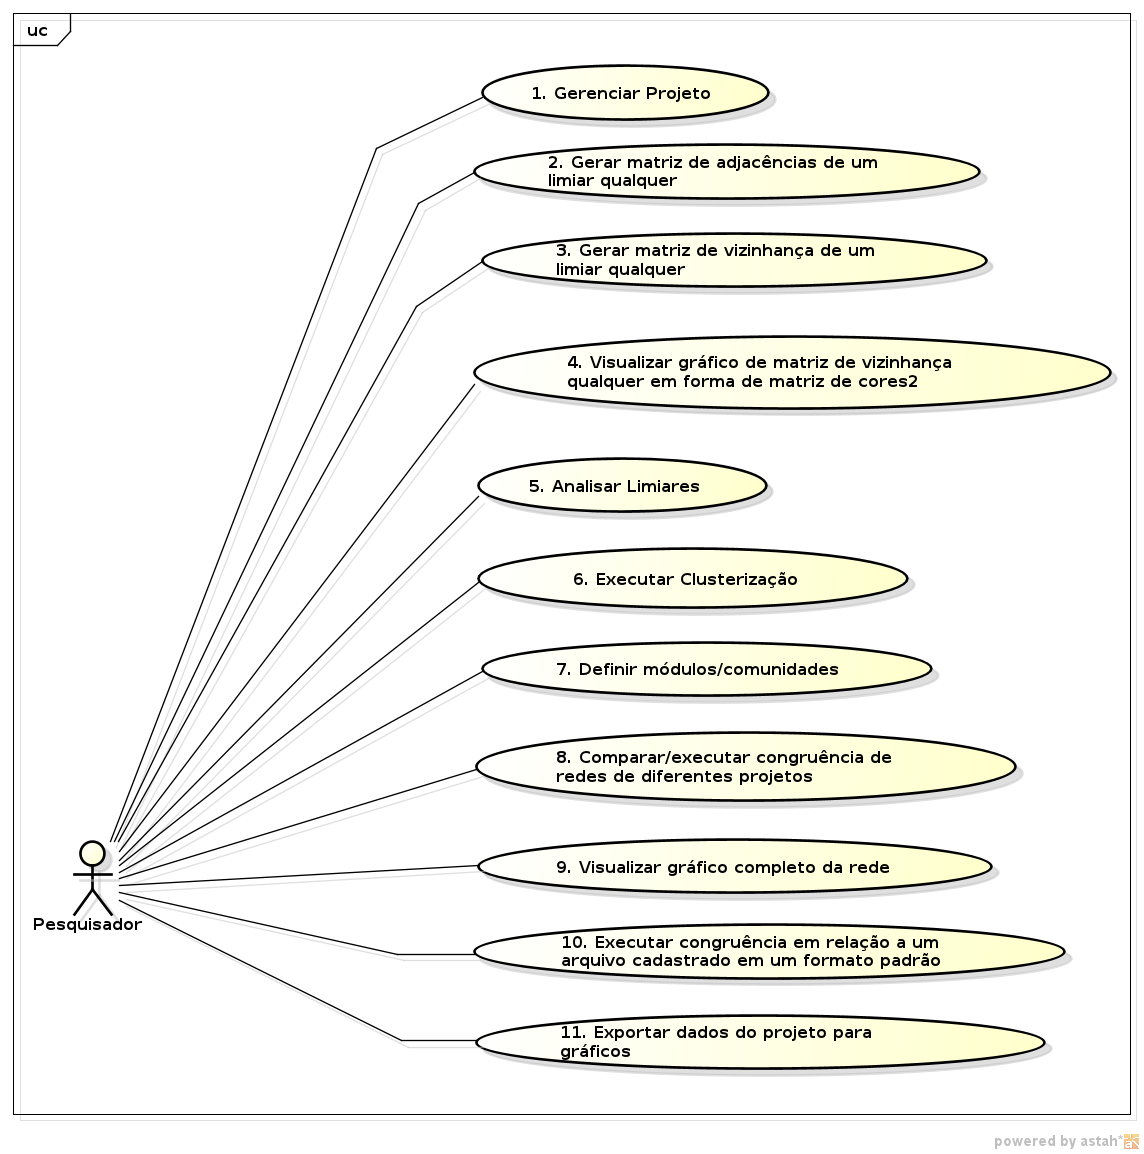
\includegraphics[scale=0.52]{diagrama-casos-de-uso}
\caption{Diagrama de casos de uso do Navi.}
\label{fig:casos-uso}
\end{figure}

Outro detalhe importante é a possibilidade de comparação entre o método e os outros métodos já consolidados de análise filogenética (através do fornecimento
de alguma arquivo em determinado formato), além de poder comparar com outro projeto criado pelo próprio sistema. A figura \ref{fig:casos-uso} exibe os casos
de uso definidos para o Navi. Para prosseguir com a modelagem, se faz necessária a organização das informações através de um diagrama de classes,
mostrado na próxima seção.

\section{Organização das Informações} \label{sec:organizacao}

A organização das informações do sistema é um passo importante para que se tenha qualidade e se atenda aos requisitos propostos. É imprescindível, portanto,
a criação de um diagrama de classes para definir entidades e suas responsabilidades, além de seus aspectos funcionais e os dados (e formatos) em que cada uma
é responsável.

Como resultado da etapa de modelagem de dados, foi criado um diagrama de classes simplificado, como pode ser visto na figura
\ref{fig:diagrama-classes-simplificado}. O diagrama de classes completo pode ser encontrado no Apêndice.

\begin{figure}
\centering
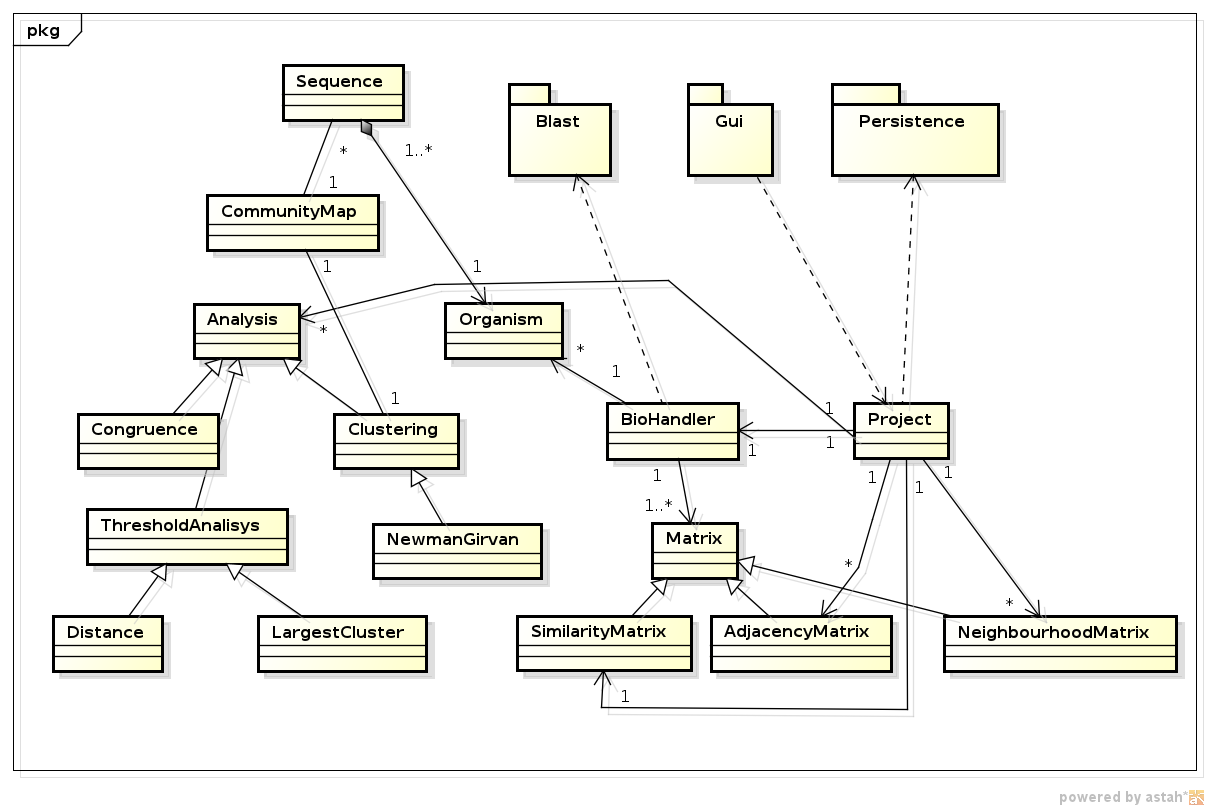
\includegraphics[scale=0.52]{diagrama-classes-simplificado}
\caption{Diagrama de classes simplificado do Navi.}
\label{fig:diagrama-classes-simplificado}
\end{figure}

A classe principal do Navi é a classe \textit{Project}. Todas as interações do usuário com a \textbf{GUI} passam por ela, que controlará operações com
matrizes, análises, tratamento das informações biológicas e dos dados de entrada. Através dela é possível criar novo projeto, abrir projeto existente e
salvar projeto corrente (casos de uso 1 e 2). Um projeto para o sistema reúne todos os dados de informações de execução de um conjunto de dados, desde a
a escolha de sequências, geração de matriz de similaridade, matrizes de adjacência e vizinhança, gráficos, definição de comunidades, clusterização,
congruência. A classe \textit{Project} também lida com o módulo \textit{Persistence}, que mapeia as classes do sistemas onde é necessário
persistir a estruturas de dados e armazenamento em disco. Sua função inclui serializar e desserializar os objetos do sistema, além de prover
a organização dos dados do projeto e compressão em um arquivo de extensão própria (.nav).

\sigla{GUI}{Graphical User Interface}

A filtragem do banco de dados biológico (sequências proteicas que estão em vários arquivos no diretório especificado pelo usuário) é realizada pela classe
\textit{BioHandler}, que a partir desta operação instancia objetosda classe \textit{Organism} e da classe \textit{Sequence}, ou seja, cria organismo e associa
sequências a eles. Então ela utiliza o pacote \textit{Blast}, que realiza as comparações entre sequências, para gerar e instanciar a matriz de similaridades.

O Navi possui três matrizes, representadas pelas classes \textit{SimilarityMatrix}, \textit{AdjacencyMatrix} e \textit{NeighbourhoodMatrix}. As três herdam
da classe \textit{Matrix} por conterem características em comum. Só é possível ter uma matriz de similaridades por projeto, pois como um projeto está associado
a execuções de determinado conjunto de sequências escolhido pelo usuário, há apenas uma matriz de similaridades possível para qualquer conjunto de sequências.
Em relação às demais (adjacência e vizinhança), é possível haver mais de uma. Se pesquisas posteriores desenvolverem outro tipo de matriz, ela poderá ser
facilmente incorporada ao sistema através da adição de uma nova classe que será uma especificação da classe \textit{Matrix}, o que explica o fato de a classe
\textit{Matrix} ser um classe abstrata. É possível gerar matrizes de adjacência ou de vizinhança, além da visualização de seus respectivos gráficos a qualquer
momento após a escolha das sequências e geração da matriz de similaridades, de acordo com os casos de uso 3, 4 e 5. A classe \textit{Project} contém métodos
para a geração das matrizes, o que pode ser visto no diagrama de classes completo. Após a geração das matrizes, a camada de persistência as salva em disco.

A classe \textit{Analysis} é uma classe abstrata que concentra todos os tipos de análises que podem ser feitas sobre as matrizes relacionadas às redes
proteicas. Existem três tipos de análises: Análise de Limiares (classe \textit{ThresholdAnalysis}), Clusterização (classe \textit{Clustering}) e
Congruência (class \textit{Congruence}). Como descrito anteriormente, existem duas formas atualmente de analisar limiares: Distâncias (classe
\textit{Distance}) e tamanho do maior cluster (\textit{LargestCluster}). Elas são subclasses de \textit{ThresholdAnalysis}, que também é abstrata. Essa
abordagem permite que outros métodos de análise de limiares possam ser adicionados de forma facilitada por meio de herança. O mesmo acontece com a
clusterização: a classe \textit{Clustering} é abstrata, e tem \textit{NewmanGirvan} como classe filha, que implementa o único método de clusterização
usado no processo até o momento (casos de uso 6 e 7).

A análise de congruência permite a comparação da divisão de comunidades entre diversos projetos executados sob o Navi, como também entre outros métodos de
análise filogenética, através do fornecimento de um arquivo em um formato padrão. Isso é possível graças à classe \textit{Congruence}, que herda da classe
\textit{Analysis} (casos de uso 8 e 10).

Outras funcionalidades extras do sistema incluem visualização do gráfico completo da rede, que utiliza a classe \textit{CommunityMap} para desenhar
os vértices que pertencem a uma mesma comunidade de determinada cor (caso de uso 9); e também a possibilidade de exportar dados do projeto para
gráficos em um formato de programas plotadores, utilizando-se de atributos de diversas classes, a depender do gráfico que se deseja (caso de uso 11).

A seção seguinte explicará com mais detalhes como se dão os fluxos de execução do sistema para gerar, guardar e recuperar os dados necessários para a
execução do método do FESC de análise filogenética usando Redes Complexas.

\section{Dinâmica de Execução do Sistema} \label{sec:dinamica}

Como discutido na seção anterior, a classe \textit{Project} é a classe principal do sistema, para onde os eventos captados pela interface gráfica são
enviados. Nesta seção serão abordados três importantes diagramas de sequência do Navi: criar novo projeto, gerar matriz de adjacência de um limiar qualquer
e analisar limiares. Outros casos de uso são bastante simples, ou são análogos a um dos três mostrados aqui, ou até mesmo não foram implementados. Será
apresentada uma ligeira discussão sobre sua dinâmica. Outros diagramas de sequência podem ser encontrados no Apêndice \textbf{[COLOCO TODOS OS OUTROS
DIAGRAMAS NO APENDICE?]}.

O primeiro diagrama de sequência, como pode ser visto na figura \ref{fig:new-project}, se refere à criação de um novo projeto. Primeiro, qualquer projeto
que esteja em execução é finalizado e a classe \textit{Persistence} salva qualquer alteração nos objetos do sistema. Uma decisão de projeto importante
é que após a instanciação de uma nova classe \textit{Project} é criado também um novo objeto \textit{BioHandler}, que já filtra os dados passados pelo
usuário, criando objetos \textit{Organism} e \textit{Sequence}. Após isto, \textit{Persistence} salva os dados do projeto.

Em seguida o usuário escolherá as sequências com que a matriz de similaridades será gerada, onde \textit{BioHandler} passará as sequências, duas a duas,
para que o pacote \textit{Blast} possa calcular as porcentagens, e então o primeiro possa montar a matriz de similaridades. Por fim, os dados do projeto
são salvos em disco pela classe de persistência. \newline

\begin{figure}
\centering
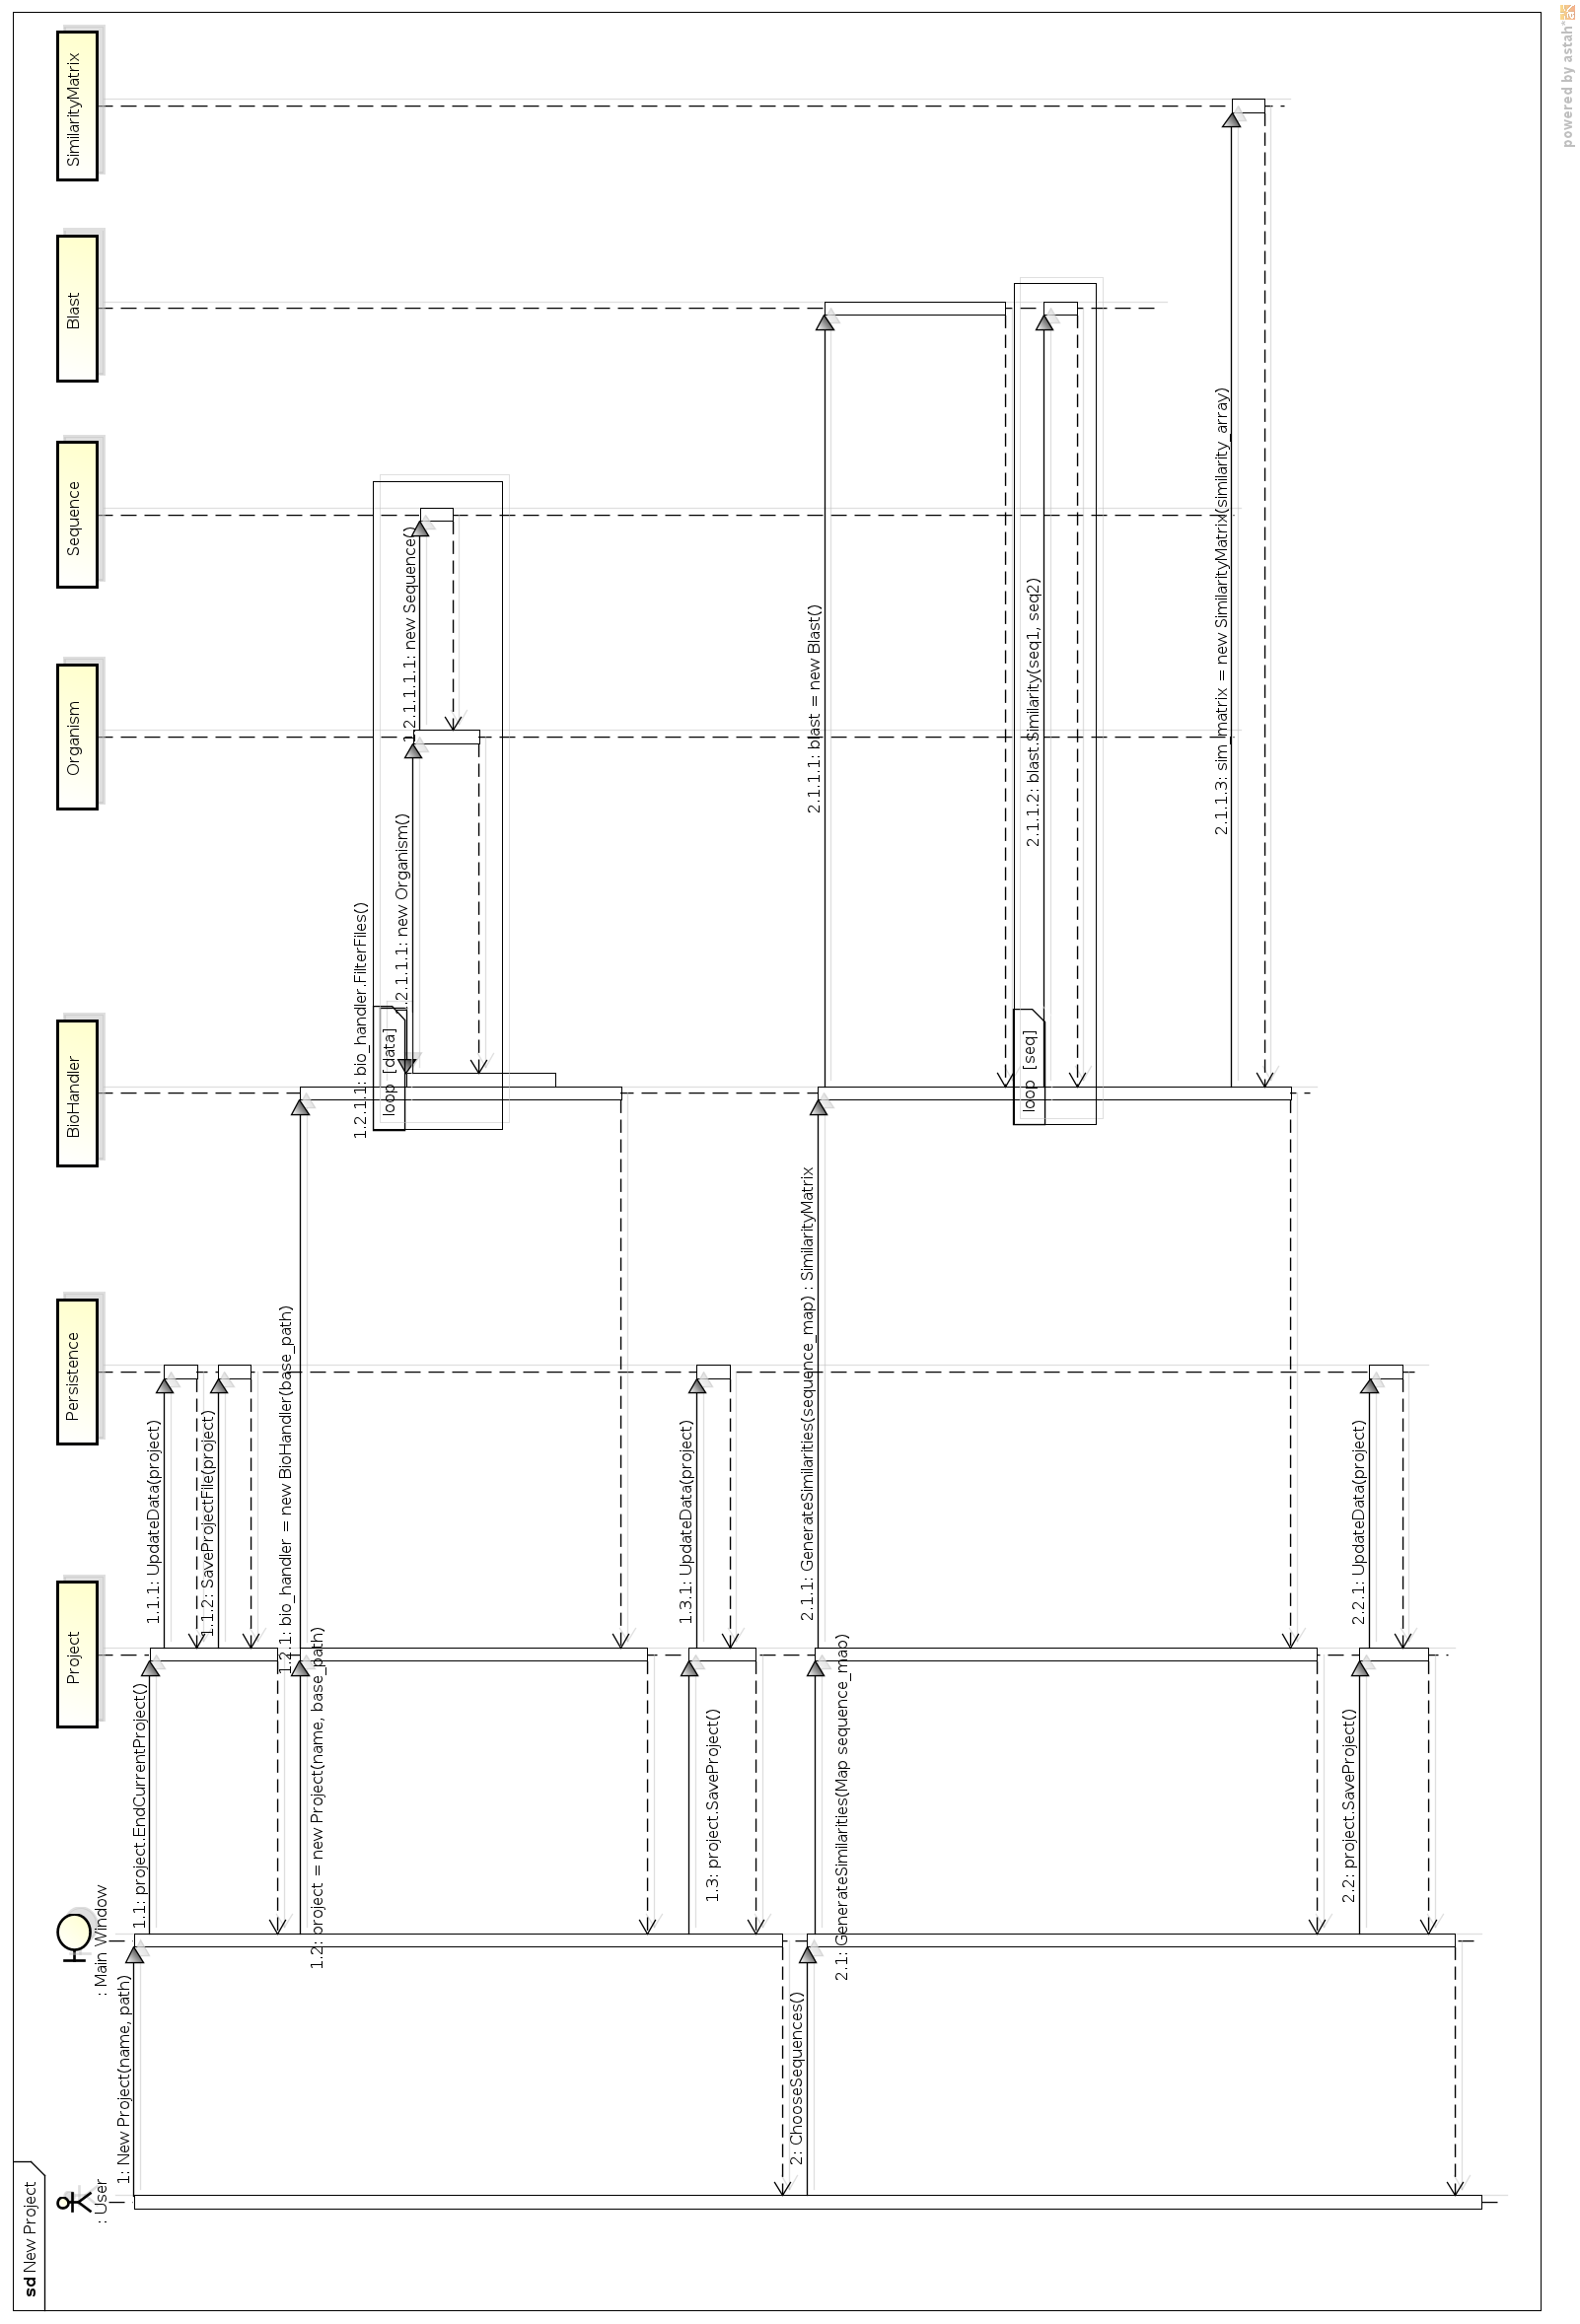
\includegraphics[scale=0.27]{new-project}
\caption{Diagrama de sequências para o requisito 1: criar novo projeto.}
\label{fig:new-project}
\end{figure}

Para gerar uma matriz de adjacências o usuário entra com um valor limiar (ou uma lista de limiares para o caso da geração de múltiplas matrizes). Haverá
então um \textit{loop} na classe \textit{Project} que instanciará objetos da classe \textit{AdjacencyMatrix}, e então usará \textit{Persistence} para salvar
novos dados em disco, conforme a figura \ref{fig:generate-adjacency-matrix}. \newline

\begin{figure}
\centering
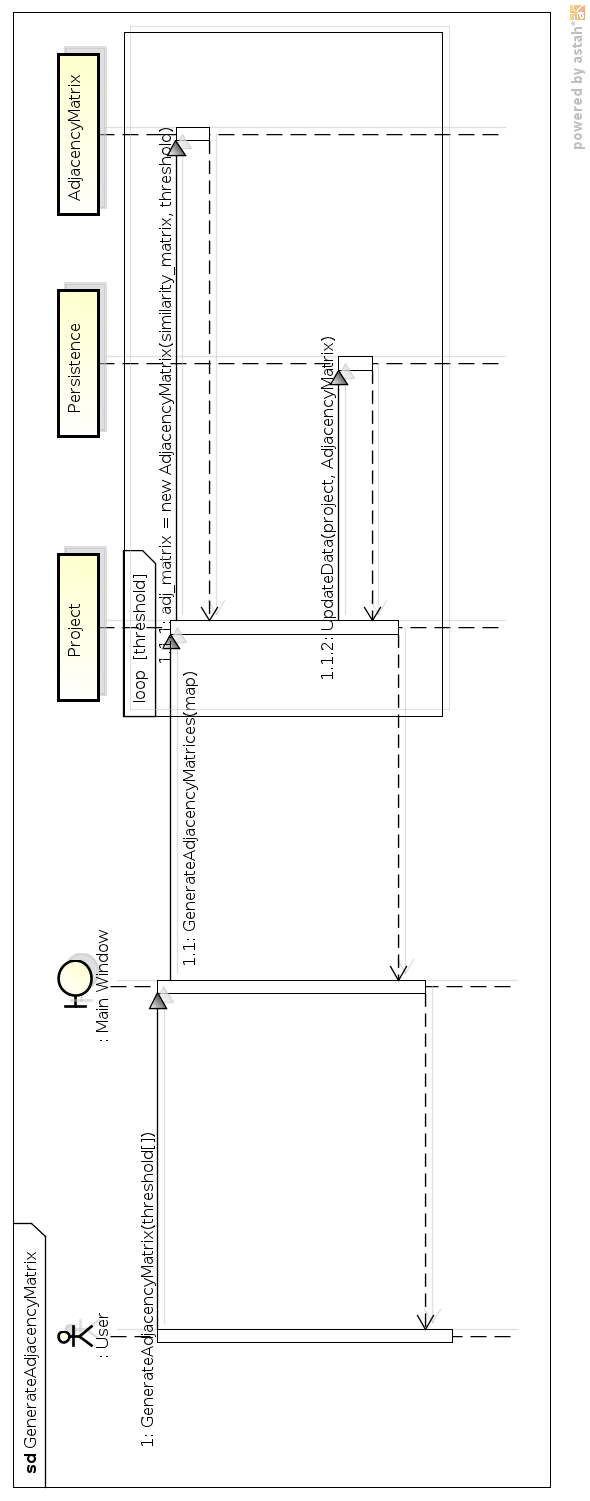
\includegraphics[scale=0.42]{generate-adjacency-matrix}
\caption{Diagrama de sequências para o requisito 3: gerar matriz de adjacências de um limiar qualquer.}
\label{fig:generate-adjacency-matrix}
\end{figure}

Para analisar limiares, o usuário precisa informar qual análise quer executar. O método do FESC de análise filogenética dispõe atualmente de dois métodos
para a realização desta análise, mas existem vários outros e que podem ser adicionados ao Navi. Atualmente o usuário deve optar, então, pelo método de
distâncias ou tamanho do maior cluster. A depender da escolha será instanciado pela classe \textit{Project} uma classe \textit{Distance} ou
\textit{LargestCluster}, respectivamente. A análise é realizada passando-se a matriz de similaridades e, ao seu final, é invocada uma biblioteca gráfica
para a exibição do gráfico para o usuário como resultado da análise. A figura \ref{fig:analyse-threshold} mostra seu diagrama de sequência. \newline

\begin{figure}
\centering
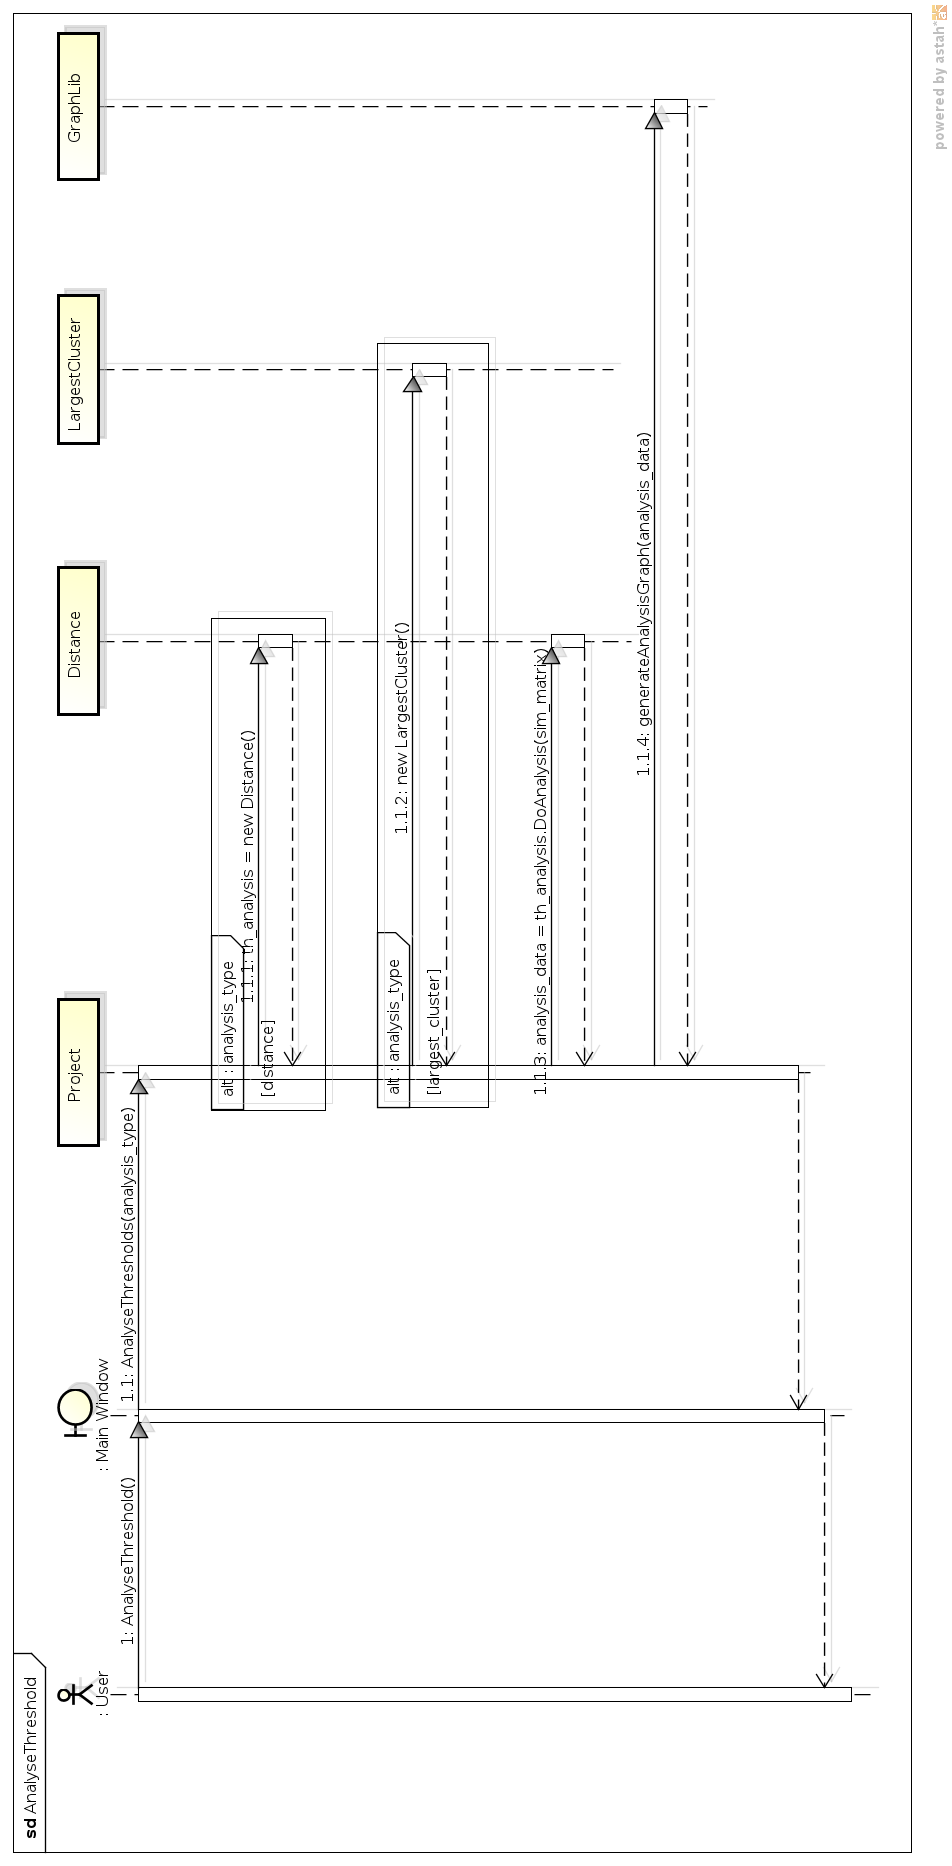
\includegraphics[scale=0.34]{analyse-threshold}
\caption{Diagrama de sequências para o requisito 6: analisar limiares.}
\label{fig:analyse-threshold}
\end{figure}

O próximo capítulo mostrará os resultados deste trabalho, seu produto gerado, as ferramentas e o ambiente de execução utilizados, características
de implementação e discutirá os resultados em relação aos objetivos propostos pelo trabalho.

\chapter{Resultados}
\label{cap:resultados}

Neste capítulo são apresentadas de forma detalhada as técnicas utilizadas para o desenvolvimento do Navi.


\section{Ambiente de execução do processo antigo} \label{sec:ambiente}

O ambiente operacional atual envolve uma série de ferramentas e linguagens: exige um ambiente GNU/Linux, um compilador Fortran, um compilador C, pacotes para
a execução de \textit{scripts} Perl e a biblioteca \textit{BioPerl}, além de um banco de dados relacional, neste caso o MySQL. Após o \textit{download} das
sequências a partir do banco de dados GenBank, as mesmas eram colocadas em um mesmo diretório, onde uma série de \textit{scripts} Perl eram executados,
realizando os seguintes passos, nesta ordem:

\begin{itemize}
  \item{Listagem de arquivos com extenção .seq, sugerindo se tratarem de arquivos do GenBank;}
  \item{Filtragem dos arquivos e armazenamento de informações importantes como Gi, locus, código da sequência na tabela SEQUENCIA do MySQL;}
  \item{Leitura dos registros da tabela SEQUENCIA, dois a dois, e execução do Blast sobre os mesmos;}
  \item{Armazenamento da porcentagem de similaridade das duas sequências na tabela SIMILARIDADE;}
  \item{Leitura da tabela SIMILARIDADE e geração de um arquivo texto contendo a matriz de similaridades.}
\end{itemize}

De posse da matriz de similaridades, é necessária a execução de outro programa para a geração das redes de diversos limiares e análise dos mesmos para que
fosse possível a escolha de um limiar crítico e então a continuação do método. Pela abordagem do tamanho do maior cluster, existe o programa achacluster,
codificado em Fortran. Para a abordagem do método das distâncias o FESC dispõe de duas alternativas: (i) a utilização do GeraRedes e em seguida o
Distância (ambos em C++); (ii) a utilização do RedeCrítica (Fortran). As duas opções têm como entrada a matriz de similaridades \footnote{O GeraRedes 
gera também as matrizes de adjacência e vizinhança e as deixa em uma pasta.} e geram um arquivo cujo formato possibilita a geração de um gráfico de pontos,
de onde é possível determinar o limiar crítico.

Utilizando então a matriz de vizinhança da rede do limiar crítico, executamos o Dendo (Fortran) que aplica o cálculo do \textit{Betweenness}, gerando como
resultado um dendrograma (histograma de remoção de arestas, indicando modularização da rede). O dendrograma, em conjunto com a matriz de cores e as sequências
permitem análises biológicas sobre os resultados.

Os módulos permanecem os mesmos, mas o controle do processo é todo gerenciado pela GUI e classes \textit{Project} e \textit{Persistence}, com auxílio de
outras classes na execução e comunicação dos módulos externos. A seção \ref{sec:discussao} detalha como se dá este gerenciamento.

\section{Ferramentas de Desenvolvimento} \label{sec:ferramentas}

A área de Bioinformática hoje em dia tem utilizado bastante Python \cite{python} no lugar de Perl para comparações entre sequências, utilização de algoritmos
genéticos, entre outras técnicas na pesquisa em geral. É uma linguagem bastante rica e poderosa, com uma grande facilidade de uso, compreensão e
desenvolvimento, rapidez na implementação e prototipagem rápida, bibliotecas robustas para o desenvolvimento de \textit{software} científico, cálculos
diversos e geração de gráficos, além de ser considerada uma ``linguagem cola'' por se comunicar facilmente com outras linguagens.

Para a criação das janelas foram testados o Tkinter (que vem com a linguagem Python), o Gtk e o Qt. O Qt foi escolhido pela sua quantidade de recursos,
facilidade de utilização, desenvolvimento e manutenção, total suporte à linguagem Python através do PyQt \cite{pyqt}, além de fornecer o \textit{Designer},
um bom ambiente de autoria para a criação de janelas e interface gráfica em geral (uma ilustração do mesmo pode ser vista na figura \ref{fig:designer}).
A utilização de Qt também permite a possibilidade de execução do Navi em ambientes Windows e Mac, faltando apenas a adaptação do \textit{back-end} para um
suporte completo a essas outras plataformas.

\begin{figure}
\centering
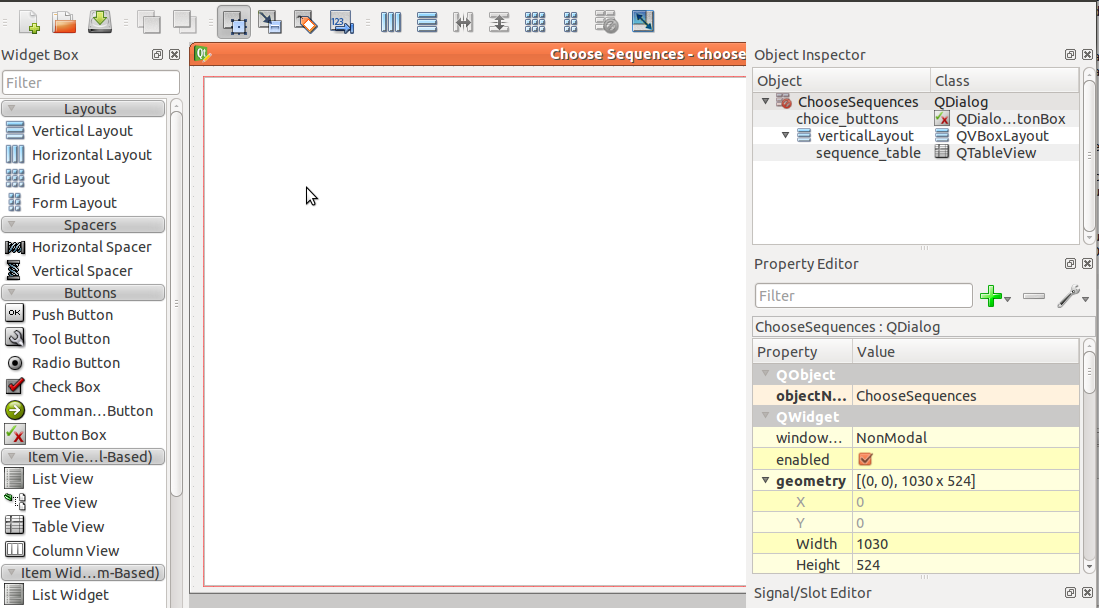
\includegraphics[scale=0.38]{designer}
\caption{Exemplo de criação de janela com o Qt4-Designer.}
\label{fig:designer}
\end{figure}

As bibliotecas necessárias e as mudanças, incluindo algumas decisões de implementação serão discutidas na próxima seção.

\section{Discussão} \label{sec:discussao}

``
Na discussão acho mais importante voce destacar as mudanças que tornam a execução de uma simulação um processo mais simples e controlado,
o que era o objetivo principal do trabalho desde o inicio!!''

A utilização da linguagem Python para o desenvolvimento do Navi acarretou certas consequências. Uma delas foi a substituição do \textit{BioPerl} pelo
\textit{BioPython} \cite{biopython}, um conjunto de ferramentas para computação biológica feito em Python, equivalente ao \textit{BioPerl} para \textit{Perl}.
Um dos gargalos na execução do método original é também a necessidade de observar gráficos e a partir deles tomar decisões relativas ao prosseguimento do
processo. Como a execução dos diversos programas era feita em Linux e o programa plotador de gŕaficos, o Origin \cite{origin} roda em Windows, em várias
situações era necessário reiniciar a máquina ou mudar de máquina para que se pudesser plotar os gráficos. Com o Matplotlib \cite{matplotlib}, biblioteca de 
plotagem de gráficos para Python, esse trabalho passa a ser desnecessário.

O \textit{BioPython} inclui o Blast2 e seus \textit{bindings} para Python. Como módulos externos, se fizeram necessários ainda o Madchar (geração de matrizes),
o RedeCrítica (análise de limiares) e o Dendo (clusterização). Por serem codificados em Fortran foi necessário o pacote Gfortran.

A primeira preocupação na implementação do Navi foi a questão inicial da filtragem e armazenamento dos dados. Um banco de dados relacional é uma exigência
muito grande para um sistema que vai realizar certos cálculos e gráficos, e que será utilizado em larga escala em máquinas diversas e por pesquisadores de
áreas como Biologia. Por isso, a primeira decisão foi a troca do banco de dados relacional por uma estrutura de armazenamento de dados através da serialização
de objetos, sendo útil também na criação de um projeto (caso de uso 1) e o carregamento de um projeto existente no disco (caso de uso 2). A classe 
\textit{Persistence} é responsável por isso, porém no protótipo o armazenamento não ficou tão bem estruturado, utilizando apenas o módulo \textit{Pickler}
do Python para a serialização de todos os objetos do sistema em um único arquivo.

Um arquivo .nav (extensão de arquivo do Navi) é simplesmente um pacote compactado que contém uma estrutura de diretórios, destinada a armazenar os arquivos
necessários à execução de um projeto, e também fornece suporte a certas operações de execução. Quando necessário, a classe \textit{Persistence} descompacta
o .nav em um diretório temporário, espera certas operações serem realizadas e então compacta novamente na localização original.

A filtragem feita originalmente não incluía uma opção de escolha das sequências com que se desejasse trabalhar. No Navi, a criação de um novo projeto resulta
na filtragem e armazenamento dos dados, e em seguida a possibilidade de escolha das sequências, como mostra a figura \ref{fig:choose-sequences}.

\begin{figure}
\centering
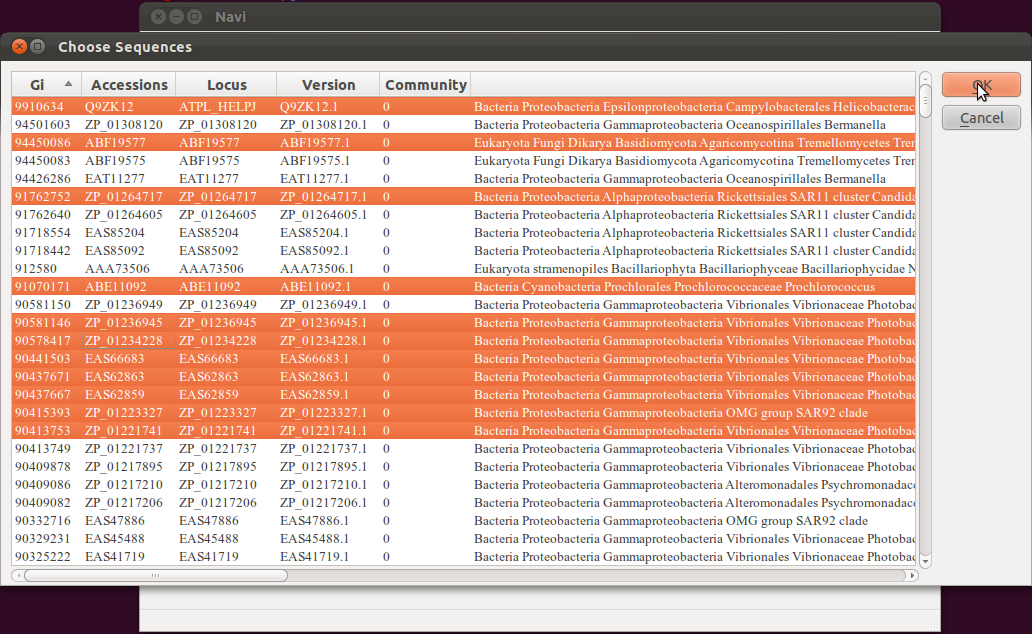
\includegraphics[scale=0.38]{choose-sequences}
\caption{Escolha das sequências no Navi após filtragem.}
\label{fig:choose-sequences}
\end{figure}

A geração de matrizes de adjacência é feita na contrução de um objeto da classe \textit{AdjacencyMatrix}, pela própria camada de negócio do Navi, sem a
necessidade de invocar módulos externos, pela simplicidade da operação. Já para gerar as matrizes de vizinhança, o módulo Madchar é invocado. A operação
também é realizada durante a construção de um objeto da classe \textit{NeighbourhoodMatrix}, onde seu construtor invoca o método
\textit{generate\_neighbourhood\_values}, que pode ser visto na listagem \ref{lst:gennbhvalues}.

``
Acho desnecessário mostrar codigo !!

Mais interessante voce mostrar a interface em vários momentos do processo.''

\lstset{language=python}
\lstset{commentstyle=\textit}
\begin{lstlisting}[frame=trbl, caption=Geração de Matriz de Adjacências,label=lst:gennbhvalues]{}
class NeighbourhoodMatrix(Matrix):
    def __init__(self, similarity_matrix, threshold):
        
        #[...]
                    
        data = self.generate_neighbourhood_values(data)
                    
        #[...]
        
    def generate_neighbourhood_values(self, adj_matrix):
        madchar_directory = tempfile.mkdtemp([...])
        
        madchar_file = os.path.join([...])
        shutil.copy(madchar_file, madchar_directory)
        
        #[...]
        
        olddir = os.getcwd()
        os.chdir(madchar_directory)
        matrix_file = open([...])
        matrix_str = ''
        for i in adj_matrix:
            for j in i:
                matrix_str += '%s' % j
            matrix_str += '\n'
        matrix_file.write(matrix_str)
        matrix_file.flush()
        subprocess.check_call(
            [os.path.join(madchar_directory,'madchar')])
        raw_nbh_matrix = open(os.path.join(madchar_directory,
            'madcharresult_11.dat'), 'r')
        os.chdir(olddir)
        
        data = raw_nbh_matrix.readlines()
        data = data[2:]
        for i in range(0, len(data)):
            data[i] = [int(j) for j in data[i].split()]
        
        raw_nbh_matrix.close()
        matrix_file.close()
        f.close()
        shutil.rmtree(madchar_directory)
        
        return data
\end{lstlisting}

A visualização do gráfico de matriz de cores se baseia nos dados da matriz de vizinhança e simplesmente os utiliza como entrada para a biblioteca
\textit{Matplotlib} desenhar o gráfico na tela.

Como explanado na seção \ref{sec:organizacao} do capítulo \ref{cap:navi}, a classe \textit{Analysis} tem a \textit{ThresholdAnalysis} como subclasse,
que por sua vez tem como classes filhas classes que representam as diferentes formas de execução da análise de limiares. Isso permite uma exetensibilidade
ao Navi, uma vez que basta acrescentar uma nova classe filha à \textit{ThresholdAnalysis} para se incluir um novo método de analisar limiares. A situação
é análoga para a clusterização, com a classe \textit{Clustering} e sua filha \textit{NewmanGirvan}.

\lstset{language=python}
\lstset{commentstyle=\textit}
\begin{lstlisting}[frame=trbl, caption=Clusterização usando o método de Newman e Girvan,label=lst:clustering]{}
class NewmanGirvan(Clustering):
    #[...]
        
    def clusterize(self, nbh_matrix):
        self.threshold = nbh_matrix.threshold
        similarity_array = nbh_matrix.data
        matrix_str = '   '
        for i in range(0, len(similarity_array)):
            for j in range(0, len(similarity_array[i])):
                matrix_str += str(similarity_array[i][j])
                if j + 1 < len(similarity_array[i]):
                    matrix_str += '   '
            matrix_str += '\n'
        
        dendo_directory = tempfile.mkdtemp([...])
        dendo_file = os.path.join([...])
        shutil.copy(dendo_file, dendo_directory)
        
        #[...]
        
        olddir = os.getcwd()
        os.chdir(dendo_directory)
        matrix_file = open([...])
        matrix_file.write(matrix_str)
        matrix_file.flush()
        
        subprocess.check_call(
            [os.path.join(dendo_directory, 'dendo')])
        
        dendrogram_file = open('d2matrixde4.dat', 'r')
        for i in dendrogram_file.readlines():
            data = [float(elem.strip('\n')) \
                for elem in i.split()]
            data = data[1:]
            self.dendrogram.append(data)
        
        os.chdir(olddir)
        
        matrix_file.close()
        f.close()
        shutil.rmtree(dendo_directory)
        
        return True
\end{lstlisting}

Nesta versão do protótipo do Navi, apenas o método de distâncias foi implementado, por meio de invocação do módulo externo RedeCrítica por um método da
classe \textit{Distance}, que é filha da classe \textit{ThresholdAnalysis}. Para a clusterização, o método de Newman e Girvan foi implementado por meio
de invocação de um módulo externo feito em Fortran (Dendo). A invocação dos módulos Fortran foi feita utilizando chamadas de sistema da linguagem Python,
que não permite uma integração perfeita, mas se utiliza do poder da linguagem de mapear as chamadas de sistema para a plataforma em que o \textit{software}
está sendo executado. A listagem \ref{lst:clustering} mostra o trecho de código que trata da invocação do módulo externo. A figura \ref{fig:navi-dendrogram}
mostra o dendrograma, resultado final do método, gerado pelo Navi.

A etapa de congruência foi modelada mas não foi implementada no protótipo por questões de tempo. Mais informações sobre a congruência podem
ser vistas em \textbf{[CITAR]}. Como o Navi não é capaz de gerar gráficos tão bons quanto uma suíte profissional dedicada à plotagem destinada a artigos e
trabalhos científicos em geral, e há perda do controle do usuário sobre a localização e o formato dos dados gerados entre as diversas etapas do processo, se
faz necessária a exportação desses arquivos para que o usuário os utilize como fonte para utilização em programas plotadores, como consta no caso de uso
12. Esta funcionalidade, no entanto, não foi implementada no protótipo.

Duas outras funcionalidades também não foram implementadas no protótipo, que são a definição de módulos/comunidades (caso de uso 8), onde o usuário define
com base na matriz de cores e no dengrograma quais sequências pertencem a quais comunidades e com isso pode ser gerado o gréfico completo da rede (caso de
uso 10) para visualização, onde o usuário pode ver as comunidades separadas por cores, além de obter facilmente informações sobre as sequências clicando nos
vértices.

\begin{figure}
\centering
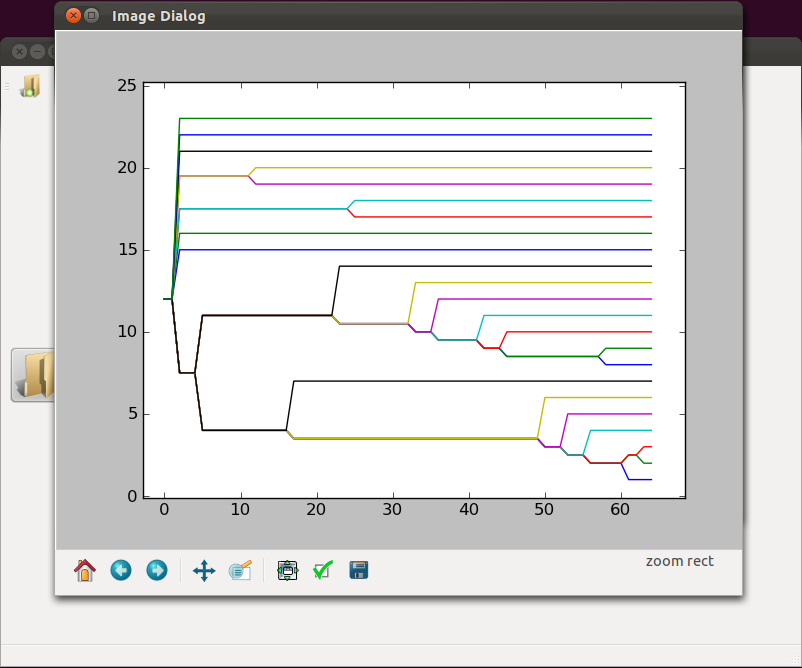
\includegraphics[scale=0.38]{navi-dendrogram}
\caption{Dendrograma mostrado pelo Navi.}
\label{fig:navi-dendrogram}
\end{figure}

\section{Dificuldades} \label{sec:dificuldades}

problemas com qt

bla



\section{Listagens} \label{sec:listagens}

\textbf{[ESSA PARTE AQUI É SUJEIRA. SÓ ESTÁ AQUI PORQUE TEM CERTOS COMANDOS QUE EU POSSO PRECISAR MAIS ADIANTE.]}

Nonono nonnono onononono \cite{fowler2000}.

Modelo de monografia usando as normas ABNT (Associao Brasileira de Normas
Tenicas) \sigla{ABNT}{Associao Brasileira de Normas Tenicas}
e adaptao personalizada 
do padro do Departamento de Cincia da Computao (DCC) da Universidade
Federal da Bahia (UFBA).
\sigla{DCC}{Departamento de Cincia da Computao}
\sigla{UFBA}{Universidade Federal da Bahia}
Fontes latex cedidos pela ABNT e disponibilizados por 
Maurcio Vieira. (Valeu Maurix!). Adaptado por Abelmon Bastos por solicitao
da \profa\ Dbora Abdalla para o semestre 2005.1.
Adaptado por Rodrigo Rocha por solicitao da \profa\ Dbora Abdalla no fim
do semestre 2007.1.

Na listagem \ref{lst:testjUnit} 
e mostrado o teste do metodo \texttt{Engine.initialize()}:

\lstset{language=java}
\lstset{commentstyle=\textit}
\begin{lstlisting}[frame=trbl, caption=Classe Factory2D,label=lst:testjUnit]{}
public class EngineTest
// JUnitDoclet begin extends_implements
extends TestCase
// JUnitDoclet end extends_implements
{
  //...
  public void testInitialize() throws Exception {
   // JUnitDoclet begin method initialize
   EngineState engineState = (EngineState) PrivateAccessor.
    getField(engine,"engineState");
   engine.initialize();
   assertEquals(engineState, new InitState());
   // JUnitDoclet end method initialize
  }
  ...
}
\end{lstlisting}

Como visto no capitulo \ref{cap:analisefilo}, no nonno\footnote{Isto e uma nota
de rodape.} no nonon onono:
\begin{itemize}
  \item{nononoo}
  \item{nononono}
  \item{no}
\end{itemize}


\section{Figuras} \label{sec:figuras}

E possivel usar imagens vetoriais no \cite{andrade2006} formato PDF, como pode ser visto
na figura \ref{fig:ufba}, ou imagens \emph{bitmap} no formato PNG, como
a da figura \ref{fig:ufba2}.

\begin{figure}
\centering

\includegraphics{brasaoUFBA2}
\caption{Brasao da UFBA (vetorial)}
\label{fig:ufba}
\end{figure}

\begin{figure}
\centering

\includegraphics[width=0.3\textwidth]{brasaoUFBA}
\caption{Brasao da UFBA (\emph{bitmap})}
\label{fig:ufba2}
\end{figure}

\chapter{Conclusao}

n ono non ono non ono ono non ononon ono non ono non ono non ono non on
 
%\section{Pontos fortes da metodologia proposta}

\section{Dificuldades encontradas}

O trabalho onon ono non ono non ono non ono non ono non on
n ono non ono non ono ono non ononon ono non ono non ono non ono non on

\section{Trabalhos futuros}

Pode-se indicar como trabalhos futuros:

\textbf{n ono non ono non ono non ono non }.
n ono non ono non ono non ono non n ono non 

ono non ono non ono non n ono non ono non ono non ono non 
\textbf{controlador} n ono non ono non ono ono non ononon ono non ono non ono non ono non on
n ono no oo non ono ononon ono  non ono non ono non ono non ono non on

\textbf{ono non ono}
o non ono non ono ono non ononon ono non ono non ono non ono non on
n ono no oo non ono ononon ono  non ono non ono non ono non ononon o 

%\section{Divulgacao}

%\section{Pontos fortes e fracos}


\appendix

\chapter{Anexo I - Diagrama de Classes completo}

\begin{figure}
\centering
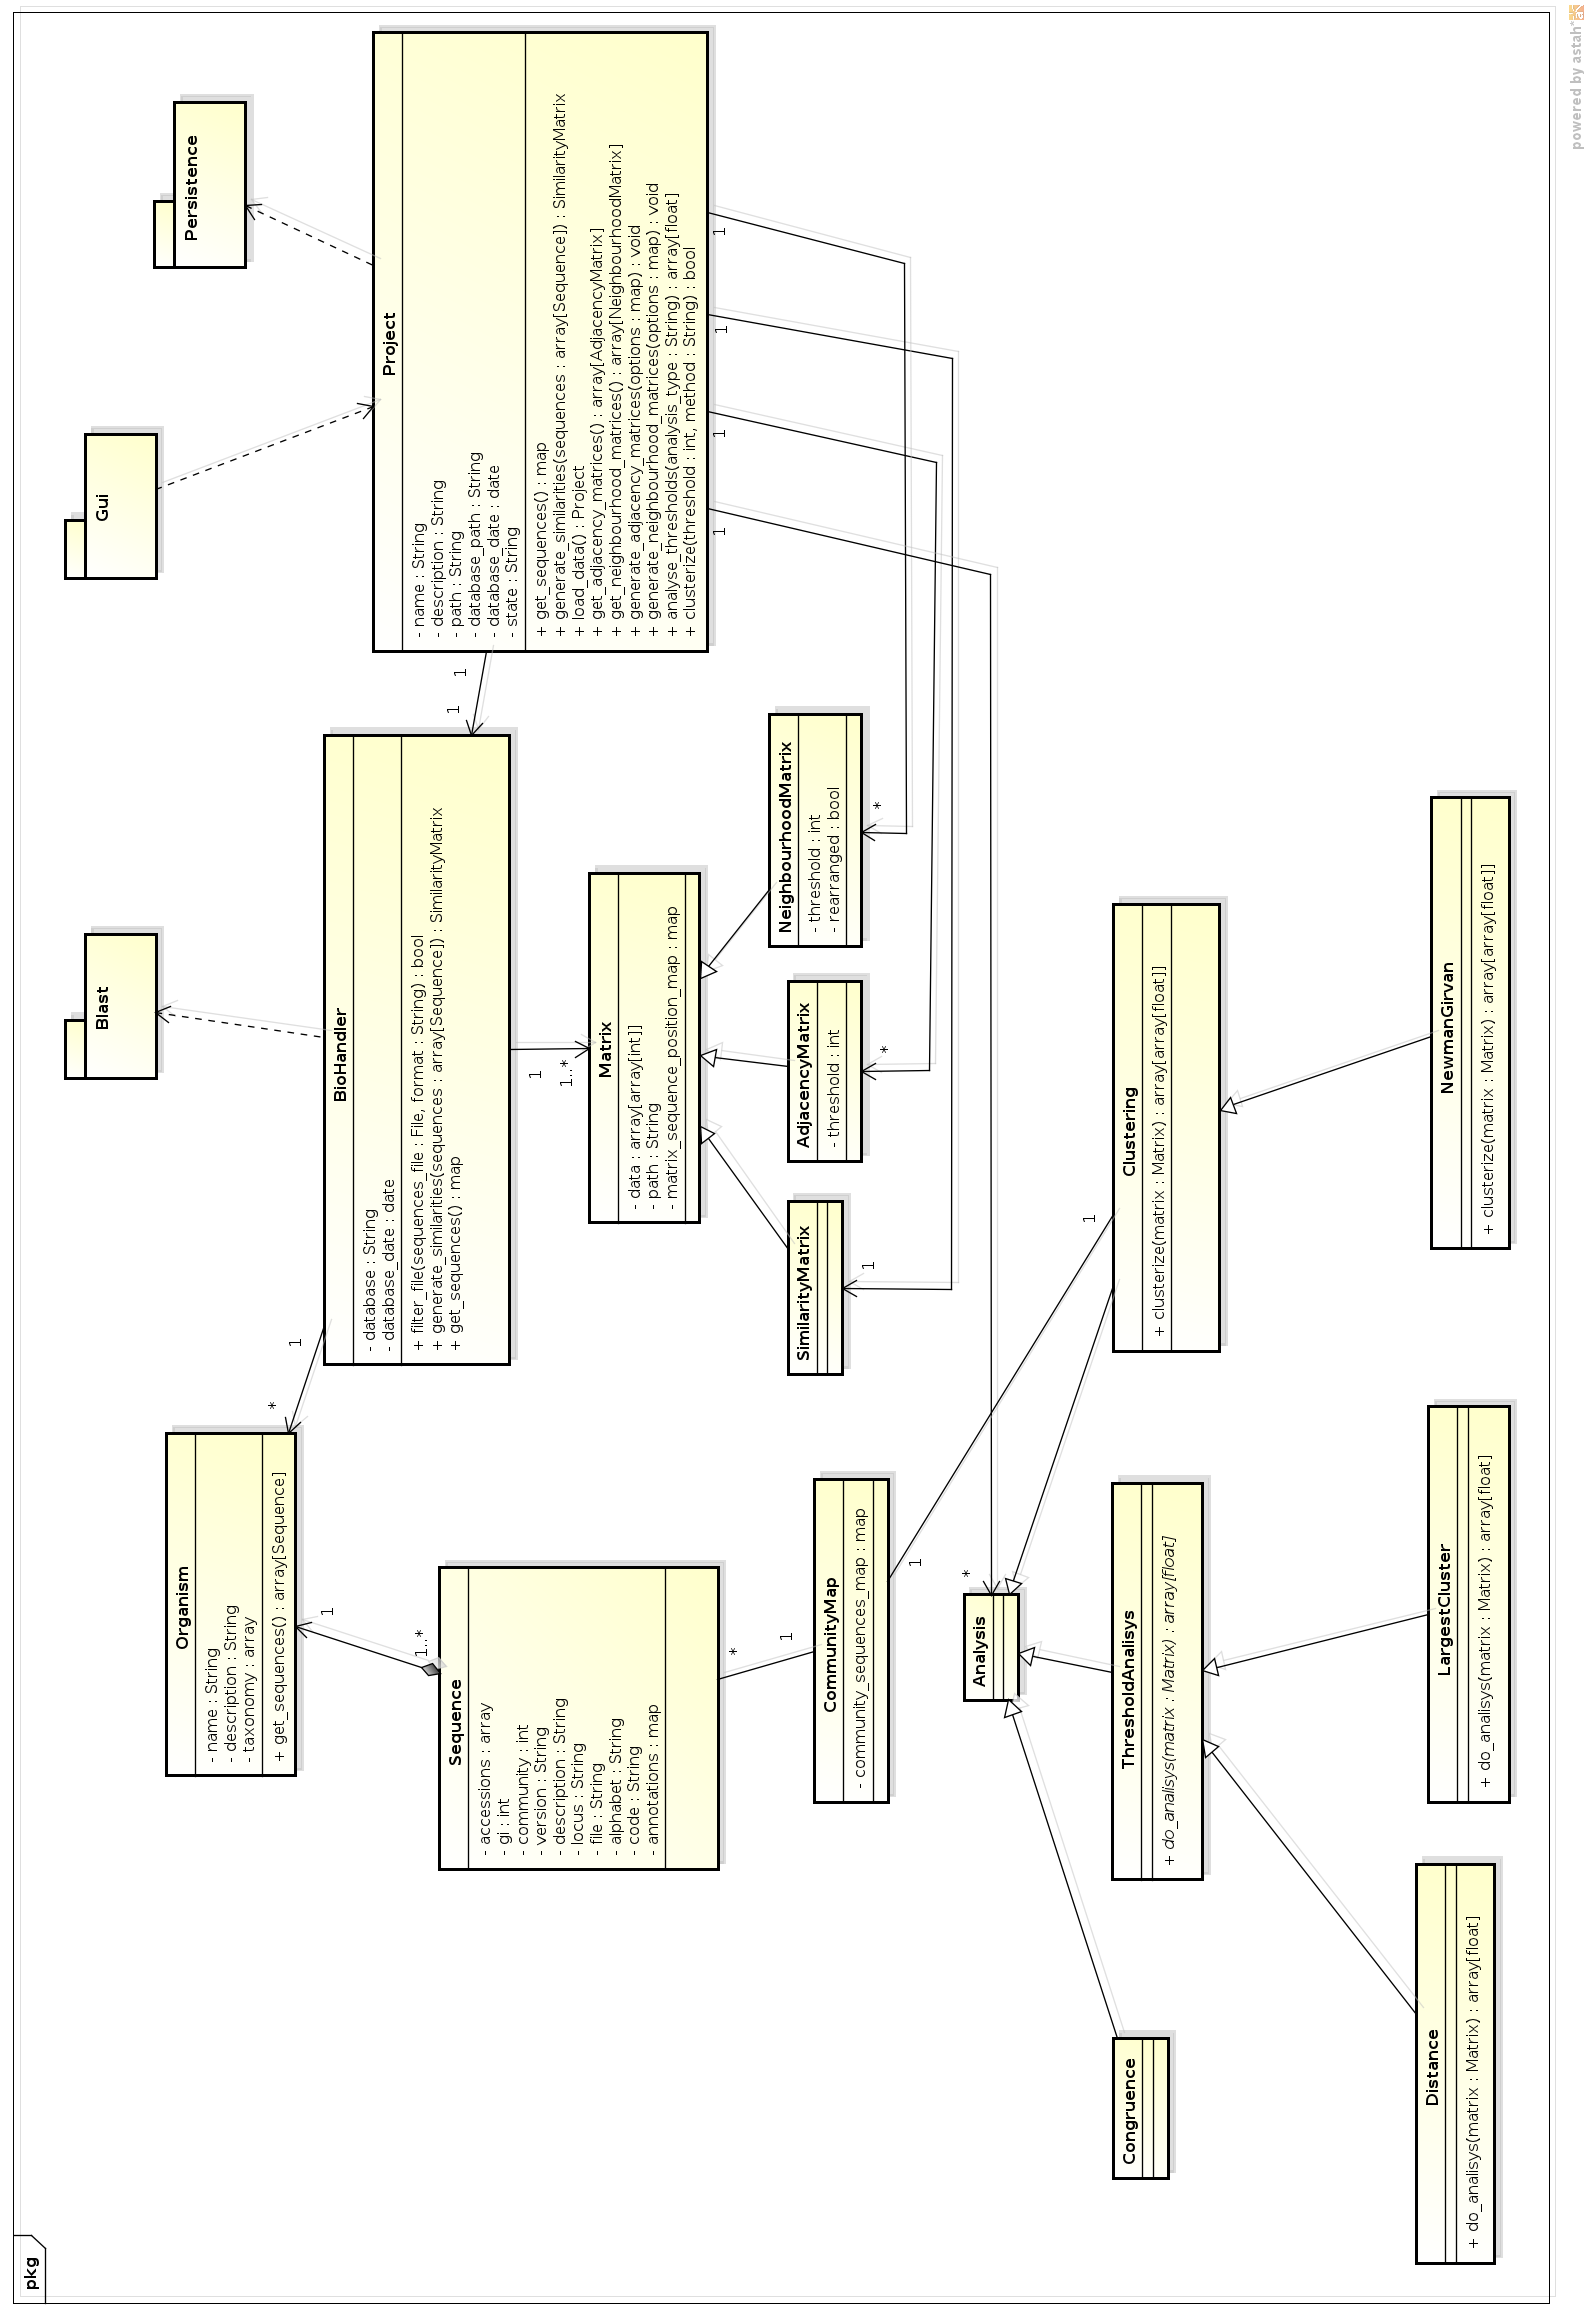
\includegraphics[scale=0.28]{diagrama-classes-completo}
\caption{Diagrama de classes completo do Navi.}
\label{fig:diagrama-classes-completo}
\end{figure}


\bibliography{monografia}

\end{document}

